% !TeX spellcheck = de_DE
\documentclass[.../Dokumentation.tex]{subfiles}
\begin{document}
\subsection{Ergebnis}\label{sec-ita4-result}
Mit den in \ref{sec-ita4-cars} vorgenommenen Änderungen am Modell konnte 
zwar genügend Platz für die Montage der kleineren Komponenten geschaffen 
werden, jedoch war der Einsatz einer Heißklebepistole erforderlich, um einen 
sicheren Halt der Bauteile zu gewährleisten.\\
Auch wenn die vertikale Anordnung der Befestigung die Problematik um das 
Stützmateri\-al löste, so konnte die in Abbildung 
\ref{fig-new-fixture-upper} gezeigte Vorrichtung die Montage nicht 
überdauern.
Da eine Erhöhung der Fülldichte bei den ohnehin schon größeren 
Fahrzeughälften die Druckzeit unverhältnismäßig verlängert hätte und die 
vorgesehenen Schächte für die Bolzen einwandfrei waren, wurde eine 
konventionellere Form der Befestigung gewählt. In den Räumen der 
Analog-Werkstatt des \textit{FabLab} fanden sich geeignete Werkzeuge. 
Nach kurzer Recherche nach den 
genauen Maßen wurden die bereits vorhandenen Löcher in der unteren Hälfte und 
die eigentlich für Bolzen vorgesehenen Schächte mittels eines Bohrers erweitert. 
In die untere Hälfte wurden nun für M3 Schrauben passende Muttern eingearbeitet. 
Unter Zuhilfenahme eines Hammers und der 
Heißklebepistole konnten diese fest mit dem Druck vereint werden. Mittels 
den Maßen des Fahrzeugs entsprechend gekürzten Schrauben war es nun möglich, 
die Hälften sicher zu vereinigen. Abbildung \ref{fig-final-fixture} zeigt das Ergebnis der hier beschriebenen 
Arbeitsschritte. Auch die transparenten Plastik-Muttern sind hier zu erkennen.
\begin{figure}[H]
\begin{center}
    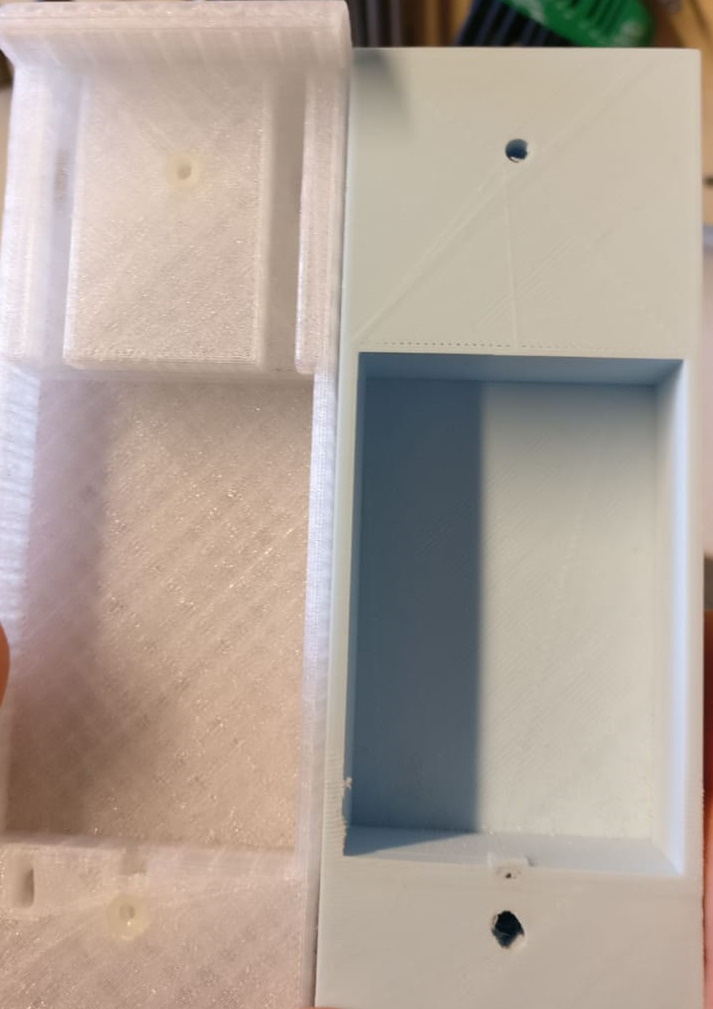
\includegraphics[
        width=0.5\linewidth,
    ]{imgs/final_fixture.jpg}
    \caption{Befestigung mit konventionellen Mitteln}
    \label{fig-final-fixture}
\end{center}
\end{figure}
\noindent 
Da das erste Fahrzeug die gestellten Anforderungen erfüllt, wurde ein weiteres 
in Form eines Busses hergestellt. Hierzu war es ausreichend, die äußere Form 
des Modells zu bearbeiten und einige Details hinzuzufügen, die den 
Wiedererkennungswert steigern. Hinsichtlich der Befestigung wurde jedoch 
gleich auf die oben ausgeführte Methode mit Schrauben und Muttern gesetzt.\\
Auch die stabileren Ausführungen von Baum und Box konnten nun montiert werden. Zunächst wurden die Äste des Baums an ihren jeweils dicksten Stellen mit einer 
feinen Holzsäge getrennt. An beiden so entstandenen Verbindungsstellen wurden 
mit einem Bohrer Löcher geschaffen, die in ihrem Durchmesser leicht über die 
Maße einer M3-Schraube hinaus gehen. Solche Schrauben wurden nun durch die 
Löcher geführt und die Äste mit Muttern in Position gebracht. 
Auf diese Weise konnten die Äste beweglich gemacht werden. 
Der Baum selbst wurde mit Hilfe eines einfachen Winkels an seiner endgültigen 
Position fixiert.
Auf die gleiche Weise wurde der in \ref{sec-ita4-visualization} erdachte 
Zwischenboden montiert. Im Anschluss konnten die Servomotoren hierauf angebracht 
werden. Um diese etwas kostspieligeren Komponenten wiederverwendbar zu halten, 
kam erneut die Klebepistole zum Einsatz.\\
Die Verbindung zwischen den Servomotoren und den Ästen, die sie bewegen sollen, 
übernahm konventioneller Faden, auch wenn die Befestigung über Knoten 
unerwartet zeitintensiv war. Der Grund hierfür war, dass es sich schwierig 
gestaltete, ein Gleichgewicht zwischen erforderlichem Halt und  
optisch ansprechender Anfangs- sowie Endposition zu finden.\\
Weiter fand die Steuerung der Visualisierung ihren Platz auf Abstandhaltern auf 
dem Zwischenboden, welche ebenfalls mit Schmelzkleber fixiert wurden.
In die Außenwand der Kiste wurde auf dieser Höhe ein Loch gebohrt, um die 
Stromversorgung ins Innere führen zu können. 
Abschließend wurde der LED-Streifen um den Baum herum montiert, wobei statt der 
oberen Hülle der Box nun die Unterseite des Zwischenbodens gewählt wurde. 
Auch hier konnte sicher gestellt werden, dass das Bauteil erneut verwendbar 
ist, indem die Befestigung mit doppelseitigem Klebeband realisiert wurde. Um den Fokus des Betrachters nicht vom Baum abzulenken, wurde weiter eine 
Blende installiert, welche die Vorgänge auf dem Zwischenboden verbirgt.\\
Die Konfiguration der Fahrzeuge und des Baums wurden zu diesem Zeitpunkt lediglich optimiert. Zusätzlich wurden für alle Komponenten Prototyp-Platinen gefertigt, welche die Montage erleichtern und eine bessere Übersichtlichkeit gewährleisten. 
\end{document}